%%%%%%%%%%%%%%%%%%%%%%%%%%%%%%%%%%%%%%%%%

% Lachaise Assignment
% LaTeX Template
% Version 1.0 (26/6/2018)
%
% This template originates from:
% http://www.LaTeXTemplates.com
%
% Authors:
% Marion Lachaise & François Févotte
% Vel (vel@LaTeXTemplates.com)
%
% License:
% CC BY-NC-SA 3.0 (http://creativecommons.org/licenses/by-nc-sa/3.0/)
% 
%%%%%%%%%%%%%%%%%%%%%%%%%%%%%%%%%%%%%%%%%

%----------------------------------------------------------------------------------------
%	PACKAGES AND OTHER DOCUMENT CONFIGURATIONS
%----------------------------------------------------------------------------------------

\documentclass[UTF8]{article}

%%%%%%%%%%%%%%%%%%%%%%%%%%%%%%%%%%%%%%%%%
% Lachaise Assignment
% Structure Specification File
% Version 1.0 (26/6/2018)
%
% This template originates from:
% http://www.LaTeXTemplates.com
%
% Authors:
% Marion Lachaise & François Févotte
% Vel (vel@LaTeXTemplates.com)
%
% License:
% CC BY-NC-SA 3.0 (http://creativecommons.org/licenses/by-nc-sa/3.0/)
% 
%%%%%%%%%%%%%%%%%%%%%%%%%%%%%%%%%%%%%%%%%

%----------------------------------------------------------------------------------------
%	PACKAGES AND OTHER DOCUMENT CONFIGURATIONS
%----------------------------------------------------------------------------------------

\usepackage{amsmath,amsfonts,stmaryrd,amssymb} % Math packages

\usepackage{enumerate} % Custom item numbers for enumerations

\usepackage[ruled]{algorithm2e} % Algorithms

\usepackage[framemethod=tikz]{mdframed} % Allows defining custom boxed/framed environments
\usepackage{cite}
\usepackage{url}
\usepackage{ctex}
\usepackage{graphicx}
\usepackage{subfigure}
\usepackage[utf8]{inputenc} % allow utf-8 input
\usepackage[T1]{fontenc}    % use 8-bit T1 fonts

\usepackage{listings} % File listings, with syntax highlighting
\lstset{
	basicstyle=\ttfamily, % Typeset listings in monospace font
}

%----------------------------------------------------------------------------------------
%	DOCUMENT MARGINS
%----------------------------------------------------------------------------------------

\usepackage{geometry} % Required for adjusting page dimensions and margins

\geometry{
	paper=a4paper, % Paper size, change to letterpaper for US letter size
	top=2.5cm, % Top margin
	bottom=3cm, % Bottom margin
	left=2.5cm, % Left margin
	right=2.5cm, % Right margin
	headheight=14pt, % Header height
	footskip=1.5cm, % Space from the bottom margin to the baseline of the footer
	headsep=1.2cm, % Space from the top margin to the baseline of the header
	%showframe, % Uncomment to show how the type block is set on the page
}

%----------------------------------------------------------------------------------------
%	FONTS
%----------------------------------------------------------------------------------------

\usepackage[utf8]{inputenc} % Required for inputting international characters
\usepackage[T1]{fontenc} % Output font encoding for international characters

\usepackage{XCharter} % Use the XCharter fonts

%----------------------------------------------------------------------------------------
%	COMMAND LINE ENVIRONMENT
%----------------------------------------------------------------------------------------

% Usage:
% \begin{commandline}
%	\begin{verbatim}
%		$ ls
%		
%		Applications	Desktop	...
%	\end{verbatim}
% \end{commandline}

\mdfdefinestyle{commandline}{
	leftmargin=10pt,
	rightmargin=10pt,
	innerleftmargin=15pt,
	middlelinecolor=black!50!white,
	middlelinewidth=2pt,
	frametitlerule=false,
	backgroundcolor=black!5!white,
	frametitle={Command Line},
	frametitlefont={\normalfont\sffamily\color{white}\hspace{-1em}},
	frametitlebackgroundcolor=black!50!white,
	nobreak,
}

% Define a custom environment for command-line snapshots
\newenvironment{commandline}{
	\medskip
	\begin{mdframed}[style=commandline]
}{
	\end{mdframed}
	\medskip
}

%----------------------------------------------------------------------------------------
%	FILE CONTENTS ENVIRONMENT
%----------------------------------------------------------------------------------------

% Usage:
% \begin{file}[optional filename, defaults to "File"]
%	File contents, for example, with a listings environment
% \end{file}

\mdfdefinestyle{file}{
	innertopmargin=1.6\baselineskip,
	innerbottommargin=0.8\baselineskip,
	topline=false, bottomline=false,
	leftline=false, rightline=false,
	leftmargin=2cm,
	rightmargin=2cm,
	singleextra={%
		\draw[fill=black!10!white](P)++(0,-1.2em)rectangle(P-|O);
		\node[anchor=north west]
		at(P-|O){\ttfamily\mdfilename};
		%
		\def\l{3em}
		\draw(O-|P)++(-\l,0)--++(\l,\l)--(P)--(P-|O)--(O)--cycle;
		\draw(O-|P)++(-\l,0)--++(0,\l)--++(\l,0);
	},
	nobreak,
}

% Define a custom environment for file contents
\newenvironment{file}[1][File]{ % Set the default filename to "File"
	\medskip
	\newcommand{\mdfilename}{#1}
	\begin{mdframed}[style=file]
}{
	\end{mdframed}
	\medskip
}

%----------------------------------------------------------------------------------------
%	NUMBERED QUESTIONS ENVIRONMENT
%----------------------------------------------------------------------------------------

% Usage:
% \begin{question}[optional title]
%	Question contents
% \end{question}

\mdfdefinestyle{question}{
	innertopmargin=1.2\baselineskip,
	innerbottommargin=0.8\baselineskip,
	roundcorner=5pt,
	nobreak,
	singleextra={%
		\draw(P-|O)node[xshift=1em,anchor=west,fill=white,draw,rounded corners=5pt]{%
		Question \theQuestion\questionTitle};
	},
}

\newcounter{Question} % Stores the current question number that gets iterated with each new question

% Define a custom environment for numbered questions
\newenvironment{question}[1][\unskip]{
	\bigskip
	\stepcounter{Question}
	\newcommand{\questionTitle}{~#1}
	\begin{mdframed}[style=question]
}{
	\end{mdframed}
	\medskip
}

%----------------------------------------------------------------------------------------
%	WARNING TEXT ENVIRONMENT
%----------------------------------------------------------------------------------------

% Usage:
% \begin{warn}[optional title, defaults to "Warning:"]
%	Contents
% \end{warn}

\mdfdefinestyle{warning}{
	topline=false, bottomline=false,
	leftline=false, rightline=false,
	nobreak,
	singleextra={%
		\draw(P-|O)++(-0.5em,0)node(tmp1){};
		\draw(P-|O)++(0.5em,0)node(tmp2){};
		\fill[black,rotate around={45:(P-|O)}](tmp1)rectangle(tmp2);
		\node at(P-|O){\color{white}\scriptsize\bf !};
		\draw[very thick](P-|O)++(0,-1em)--(O);%--(O-|P);
	}
}

% Define a custom environment for warning text
\newenvironment{warn}[1][Warning:]{ % Set the default warning to "Warning:"
	\medskip
	\begin{mdframed}[style=warning]
		\noindent{\textbf{#1}}
}{
	\end{mdframed}
}

%----------------------------------------------------------------------------------------
%	INFORMATION ENVIRONMENT
%----------------------------------------------------------------------------------------

% Usage:
% \begin{info}[optional title, defaults to "Info:"]
% 	contents
% 	\end{info}

\mdfdefinestyle{info}{%
	topline=false, bottomline=false,
	leftline=false, rightline=false,
	nobreak,
	singleextra={%
		\fill[black](P-|O)circle[radius=0.4em];
		\node at(P-|O){\color{white}\scriptsize\bf i};
		\draw[very thick](P-|O)++(0,-0.8em)--(O);%--(O-|P);
	}
}

% Define a custom environment for information
\newenvironment{info}[1][Info:]{ % Set the default title to "Info:"
	\medskip
	\begin{mdframed}[style=info]
		\noindent{\textbf{#1}}
}{
	\end{mdframed}
}
 % Include the file specifying the document structure and custom commands
\usepackage{multirow}
%----------------------------------------------------------------------------------------
%	ASSIGNMENT INFORMATION
%----------------------------------------------------------------------------------------

\title{Introduction to HPC \\ HW5 Report} % Title of the assignment

\author{姓名:任一  \\学号:2018011423\\ \texttt{ry18@mails.tsinghua.edu.cn}} % Author name and email address

\date{\today} % University, school and/or department name(s) and a date

%----------------------------------------------------------------------------------------
\lstset{
    % backgroundcolor=\color{red!50!green!50!blue!50},%代码块背景色为浅灰色
    rulesepcolor= \color{gray}, %代码块边框颜色
    breaklines=true,  %代码过长则换行
    numbers=left, %行号在左侧显示
    numberstyle= \small,%行号字体
    keywordstyle= \color{blue},%关键字颜色
    commentstyle=\color{gray}, %注释颜色
    frame=shadowbox%用方框框住代码块
}

\begin{document}

\maketitle % Print the title
\begin{center}
    \begin{tabular}{l  r}
    \hline
        \multicolumn{2}{c}{实验环境} \\ \hline
        操作系统: & Windows10家庭版 18362.72 Windows Subsystem for Linux \\ \hline% Date the experiment was performed
        gcc版本: & gcc version 7.5.0 \\ \hline% Partner names
        集群处理器:&Intel(R) Xeon(R)  E5-2680 v3\\ \hline
        集群核心数:&24\\ \hline
    \end{tabular}
\end{center}
\newpage

\section{Exercise5.4}
各规约操作符与其初始化的变量值如下表:
\begin{table}[h]
    \label{tab:my-table}
    \centering
    \caption{规约运算符与其对应的变量初始值表}
    \begin{tabular}{|l|l|}
    \hline
    Operator           & Initial Value \\ \hline
    \&\&               & $1$             \\ \hline
    ||                 & $0$             \\ \hline
    \&                 & $111...111_2$     \\ \hline
    |                  & $0$             \\ \hline
    \textasciicircum{} & $0$             \\ \hline
    \end{tabular}
    \end{table}

\section{Exercise5.5}
\subsection{1}
串行相加时,当完成最后一次相加后,寄存器中的数值是$1.008e+03$, 
当这个数字被存储到内存中时,该数值被四舍五入为3位十进制有效数字,
即$sum = 1.01e+03$. 因此输出的值为1010.0.

\subsection{2}
使用2线程并行相加时,
0号线程负责前两个数的相加,局部和为$4.00e+00$, 1号线程负责后两个数
的相加,局部和为$1.00e+03$(此处发生了四舍五入). 
这两个线程局部和相加,得到的结果为$1.00+03$(此处发生了四舍五入).
因此输出的值为$1000.0$.
\clearpage

\section{PA1}
本题中我主要使用了parallel for语句,使得每一个Process
中都采用了OMP的并行方式。

本题在集群上的目录为/home/2018011423/HW5/PA1,在该文件夹下输入make即可编译,make run即可运行。

\subsection{并行串行结果之差二范数}
在所有测试中,我的并行结果与串行结果之差的二范数都是0,这体现出了我的并行程序的正确性。
\subsection{矩阵乘法与二范数计算时间分析}
% Please add the following required packages to your document preamble:
% \usepackage{multirow}
\subsubsection{矩阵乘法计算时间}
\begin{table}[h]
    \caption{并行计算时间表}
    \label{tab:my-table}
    \centering
    \begin{tabular}{|c|l|l|l|l|}
    \hline
    \multicolumn{5}{|c|}{parallel calc time}                                                                                \\ \hline
    \multicolumn{1}{|l|}{}                                                 &            & \multicolumn{3}{c|}{MATRIX ORDER} \\ \hline
    \multicolumn{1}{|l|}{}                                                 & Processors & 2160      & 4320      & 7200      \\ \hline
    \multirow{3}{*}{\begin{tabular}[c]{@{}c@{}}10 \\ THREADS\end{tabular}} & 4          & 0.012486  & 0.017767  & 0.028428  \\ \cline{2-5} 
                                                                           & 9          & 0.027715  & 0.027137  & 0.038875  \\ \cline{2-5} 
                                                                           & 16         & 0.045799  & 0.04003   & 0.053367  \\ \hline
    \multirow{3}{*}{\begin{tabular}[c]{@{}c@{}}20 \\ THREADS\end{tabular}} & 4          & 0.021975  & 0.02776   & 0.038028  \\ \cline{2-5} 
                                                                           & 9          & 0.050516  & 0.050927  & 0.062229  \\ \cline{2-5} 
                                                                           & 16         & 0.086376  & 0.082736  & 0.092697  \\ \hline
    \end{tabular}
    \end{table}
    \begin{figure}[h]
        \label{Ratio}
        \centering
            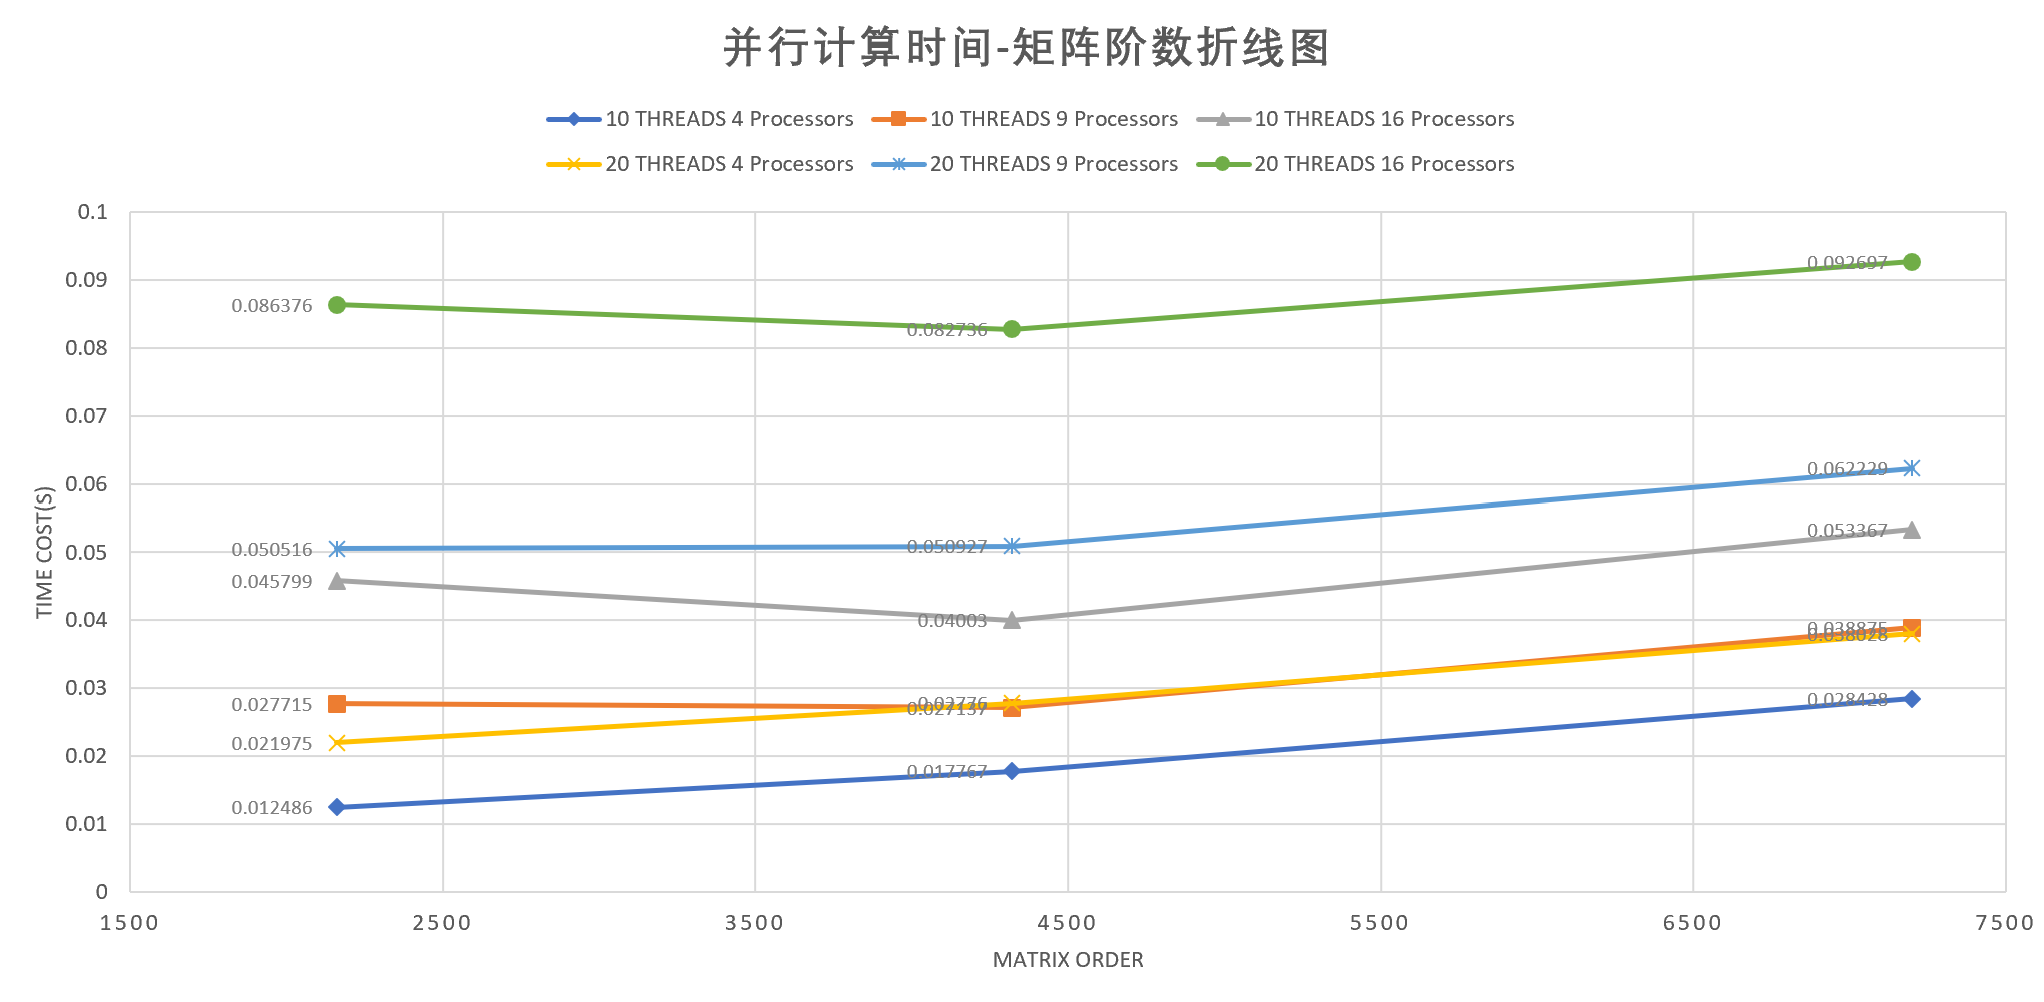
\includegraphics[width=0.8\textwidth]{pct.png}
            \caption{并行计算时间与矩阵阶数折线图}
        \end{figure}
    \clearpage
\subsubsection{二范数计算时间}

        \begin{table}[h]
            \caption{二范数计算时间表}
            \label{tab:my-table}
            \centering
            \begin{tabular}{|l|l|l|l|}
            \hline
                       & \multicolumn{3}{c|}{L2 Norm Calc Time} \\ \hline
                       & 2160        & 4320        & 7200       \\ \hline
            SERIAL     & 0.000007    & 0.000013    & 0.000021   \\ \hline
            10 THREADS & 0.000058    & 0.00006     & 0.00008    \\ \hline
            20 THREADS & 0.000085    & 0.002227    & 0.006091   \\ \hline
            \end{tabular}
            \end{table}
            \begin{figure}[h]
                \label{Ratio}
                \centering
                    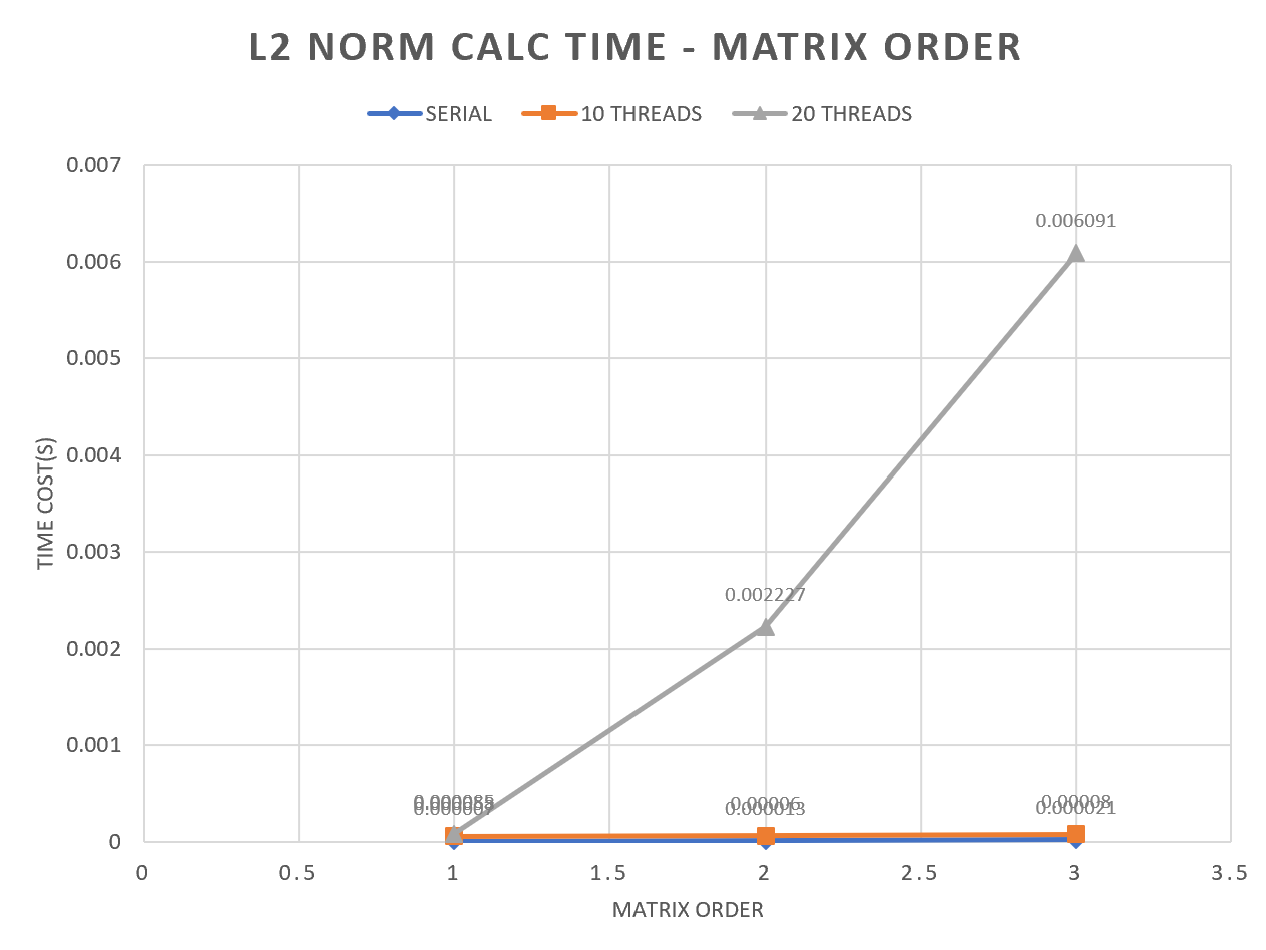
\includegraphics[width=0.8\textwidth]{lct.png}
                    \caption{二范数计算时间折线图}
                \end{figure}
从图中可以明显看出,多线程对于二范数计算的加速并不明显。原因可能是二范数计算范围较小,
线程的开辟和回收时间成本可能大于并行带来的时间收益。
\clearpage
\subsection{并行总时间、计算时间、通信时间、加速比、并行效率}
\subsubsection{并行总时间}
% Please add the following required packages to your document preamble:
% \usepackage{multirow}
% \usepackage[table,xcdraw]{xcolor}
% If you use beamer only pass "xcolor=table" option, i.e. \documentclass[xcolor=table]{beamer}
\begin{table}[h]
    \caption{并行总时间表}
    \label{tab:my-table}
    \centering
    \begin{tabular}{|c|l|l|l|l|}
    \hline
    \multicolumn{5}{|c|}{parallel all time}                                                                                                                                                    \\ \hline
    \multicolumn{1}{|l|}{}                                                  &            & \multicolumn{3}{c|}{MATRIX ORDER}                                                                   \\ \hline
    \multicolumn{1}{|l|}{}                                                  & Processors & 2160                            & 4320                            & 7200                            \\ \hline
                                                                            & 4          & {\color[HTML]{000000} 0.125707} & {\color[HTML]{000000} 0.343842} & {\color[HTML]{000000} 0.822637} \\ \cline{2-5} 
                                                                            & 9          & {\color[HTML]{000000} 0.134293} & {\color[HTML]{000000} 0.368953} & {\color[HTML]{000000} 0.905315} \\ \cline{2-5} 
    \multirow{-3}{*}{\begin{tabular}[c]{@{}c@{}}10 \\ THREADS\end{tabular}} & 16         & {\color[HTML]{000000} 0.164941} & {\color[HTML]{000000} 0.39197}  & {\color[HTML]{000000} 0.942639} \\ \hline
                                                                            & 4          & {\color[HTML]{000000} 0.135145} & {\color[HTML]{000000} 0.36316}  & {\color[HTML]{000000} 0.884623} \\ \cline{2-5} 
                                                                            & 9          & {\color[HTML]{000000} 0.167472} & {\color[HTML]{000000} 0.386904} & {\color[HTML]{000000} 0.9313}   \\ \cline{2-5} 
    \multirow{-3}{*}{\begin{tabular}[c]{@{}c@{}}20 \\ THREADS\end{tabular}} & 16         & {\color[HTML]{000000} 0.204671} & {\color[HTML]{000000} 0.432752} & {\color[HTML]{000000} 0.961524} \\ \hline
    \end{tabular}
    \end{table}
    \begin{figure}[h]
        \label{Ratio}
        \centering
            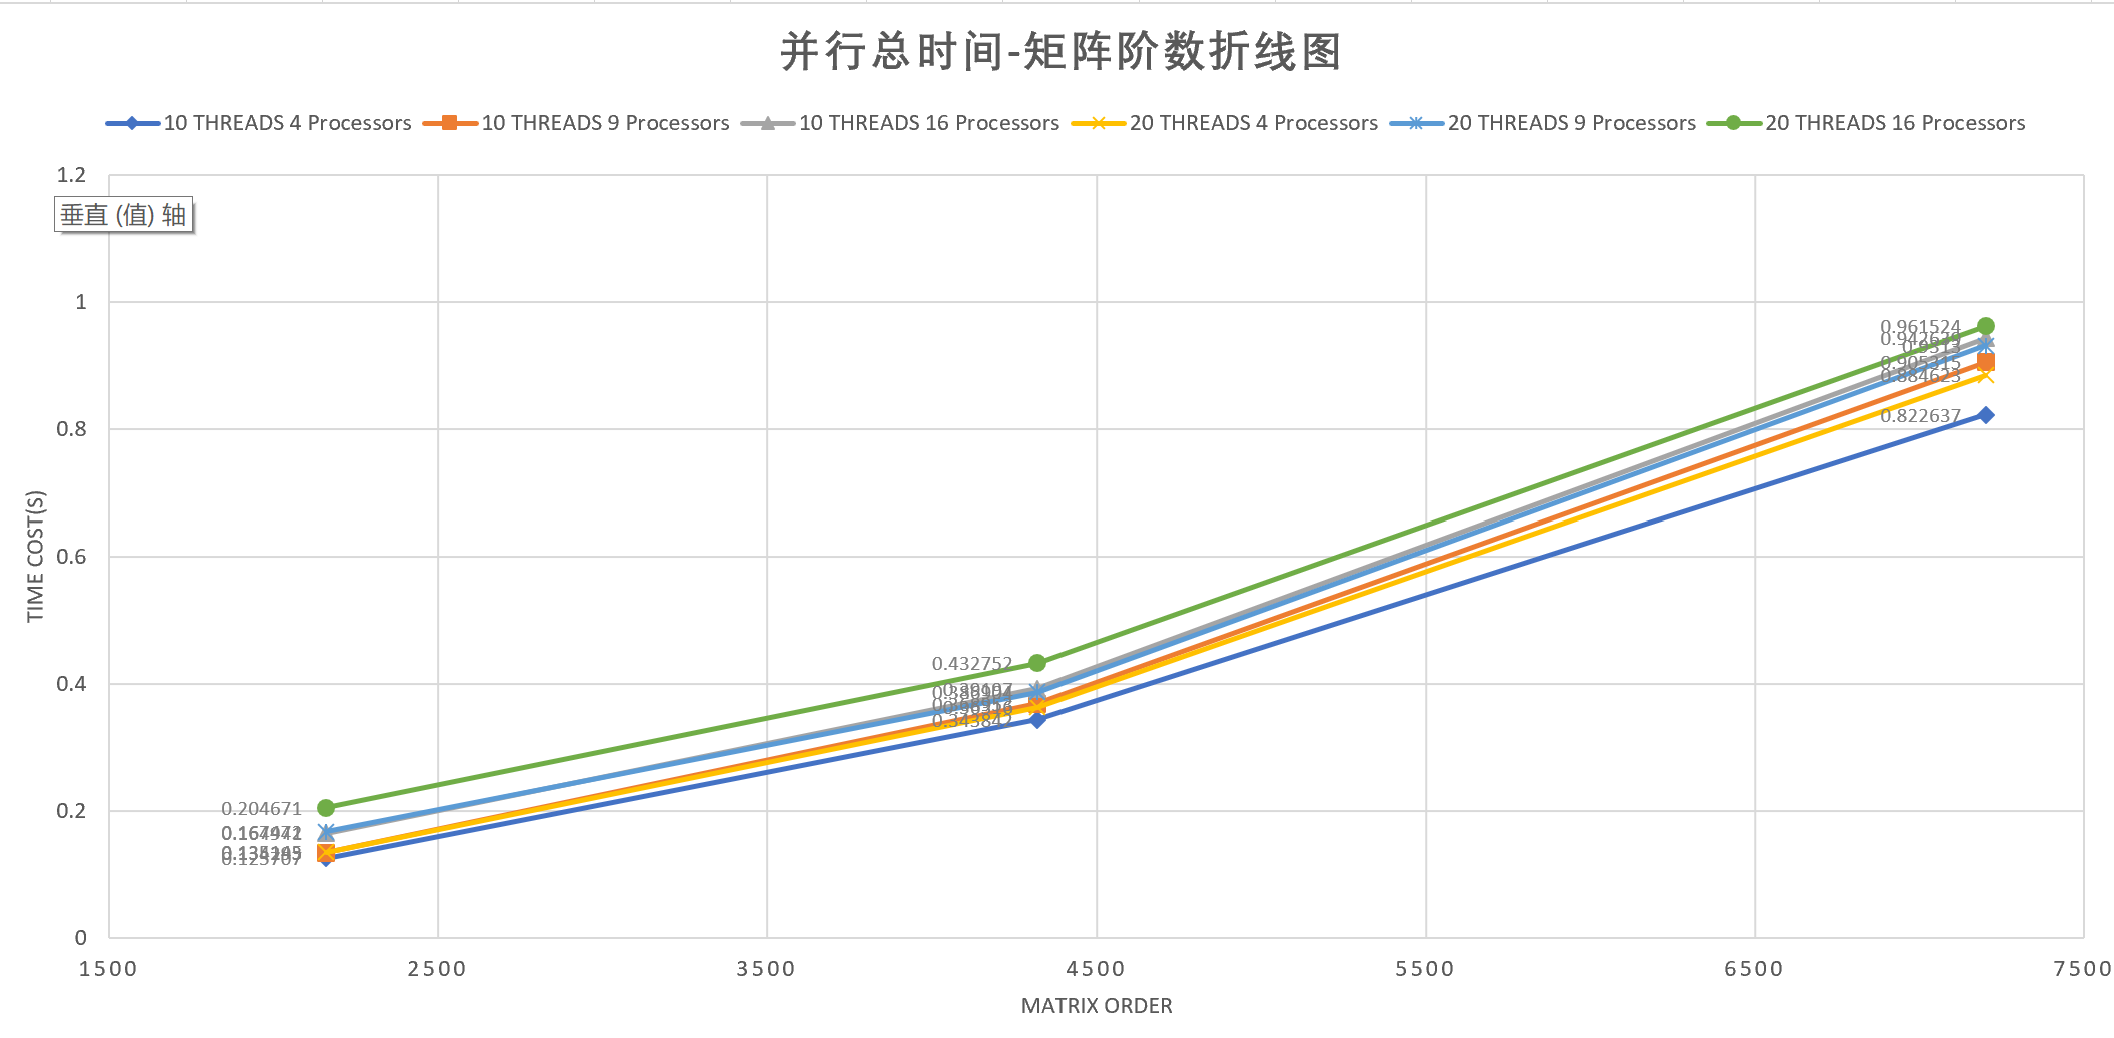
\includegraphics[width=0.8\textwidth]{pal.png}
            \caption{并行总时间折线图}
        \end{figure}
\clearpage

\subsubsection{并行计算时间}
并行计算时间的图表已经在4.1中分析了,在此不再重复。
\subsubsection{并行通信时间}
% Please add the following required packages to your document preamble:
% \usepackage{multirow}
% \usepackage[table,xcdraw]{xcolor}
% If you use beamer only pass "xcolor=table" option, i.e. \documentclass[xcolor=table]{beamer}
\begin{table}[h]
    \caption{并行通信时间表}
    \label{tab:my-table}
    \centering

    \begin{tabular}{|c|l|l|l|l|}
    \hline
    \multicolumn{5}{|c|}{parallel distribution time}                                                                                                                                           \\ \hline
    \multicolumn{1}{|l|}{}                                                  &            & \multicolumn{3}{c|}{MATRIX ORDER}                                                                   \\ \hline
    \multicolumn{1}{|l|}{}                                                  & Processors & 2160                            & 4320                            & 7200                            \\ \hline
                                                                            & 4          & {\color[HTML]{000000} 0.113221} & {\color[HTML]{000000} 0.326075} & {\color[HTML]{000000} 0.794209} \\ \cline{2-5} 
                                                                            & 9          & {\color[HTML]{000000} 0.106578} & {\color[HTML]{000000} 0.341816} & {\color[HTML]{000000} 0.866440} \\ \cline{2-5} 
    \multirow{-3}{*}{\begin{tabular}[c]{@{}c@{}}10 \\ THREADS\end{tabular}} & 16         & {\color[HTML]{000000} 0.119142} & {\color[HTML]{000000} 0.351940} & {\color[HTML]{000000} 0.889272} \\ \hline
                                                                            & 4          & {\color[HTML]{000000} 0.11317}  & {\color[HTML]{000000} 0.3354}   & {\color[HTML]{000000} 0.846595} \\ \cline{2-5} 
                                                                            & 9          & {\color[HTML]{000000} 0.116956} & {\color[HTML]{000000} 0.335977} & {\color[HTML]{000000} 0.869071} \\ \cline{2-5} 
    \multirow{-3}{*}{\begin{tabular}[c]{@{}c@{}}20 \\ THREADS\end{tabular}} & 16         & {\color[HTML]{000000} 0.118295} & {\color[HTML]{000000} 0.350016} & {\color[HTML]{000000} 0.868827} \\ \hline
    \end{tabular}
    \end{table}

    \begin{figure}[h]
        \label{Ratio}
        \centering
            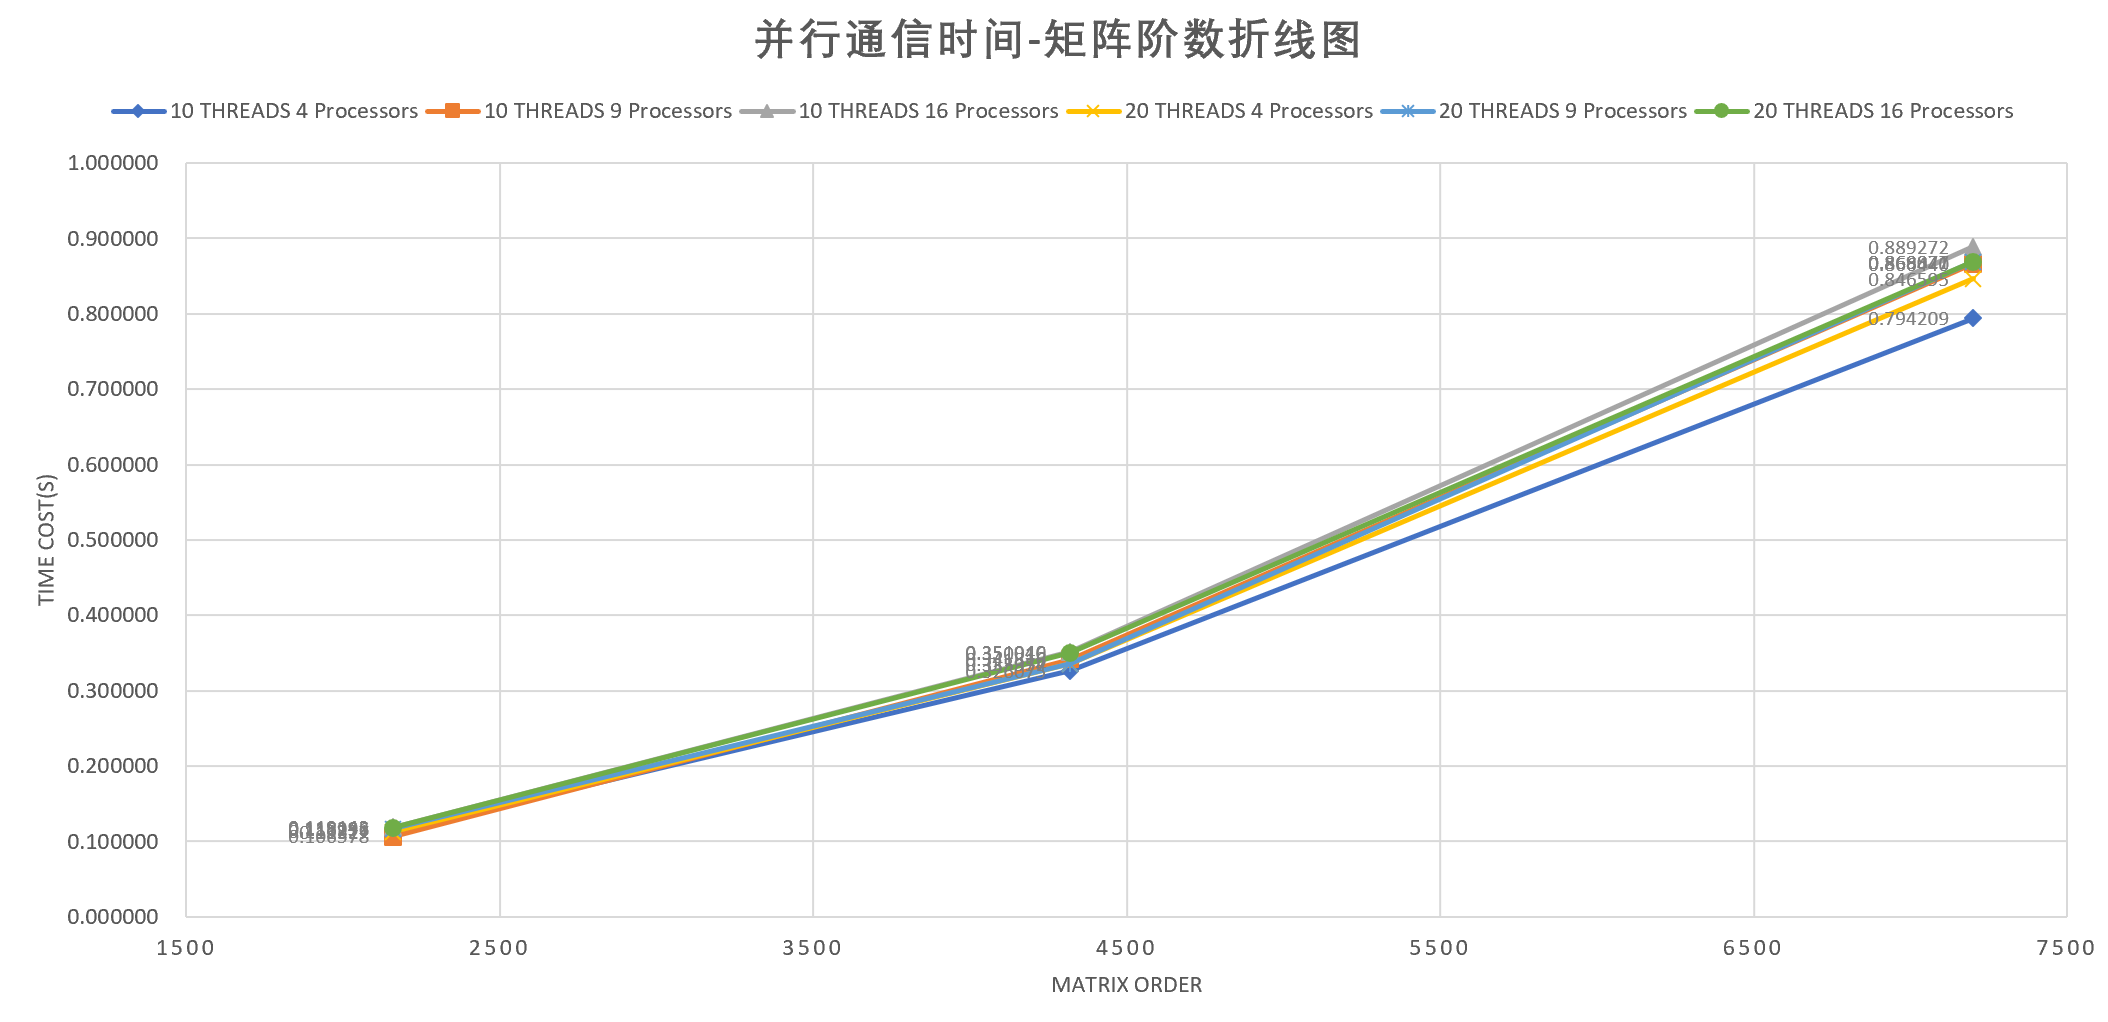
\includegraphics[width=0.8\textwidth]{pdt.png}
            \caption{并行通信时间折线图}
        \end{figure}
\clearpage

\subsubsection{并行计算时间加速比}
% Please add the following required packages to your document preamble:
% \usepackage{multirow}
% \usepackage[table,xcdraw]{xcolor}
% If you use beamer only pass "xcolor=table" option, i.e. \documentclass[xcolor=table]{beamer}
\begin{table}[h]
    \caption{并行加速比表}
    \label{tab:my-table}
    \centering

    \begin{tabular}{|c|l|l|l|l|}
    \hline
    \multicolumn{5}{|c|}{parallel speed up ratio}                                                                                                                                              \\ \hline
    \multicolumn{1}{|l|}{}                                                  &            & \multicolumn{3}{c|}{MATRIX ORDER}                                                                   \\ \hline
    \multicolumn{1}{|l|}{}                                                  & Processors & 2160                            & 4320                            & 7200                            \\ \hline
                                                                            & 4          & {\color[HTML]{000000} 2.607801} & {\color[HTML]{000000} 3.233748} & {\color[HTML]{000000} 5.584881} \\ \cline{2-5} 
                                                                            & 9          & {\color[HTML]{000000} 1.051633} & {\color[HTML]{000000} 2.385046} & {\color[HTML]{000000} 4.616875} \\ \cline{2-5} 
    \multirow{-3}{*}{\begin{tabular}[c]{@{}c@{}}10 \\ THREADS\end{tabular}} & 16         & {\color[HTML]{000000} 0.353610} & {\color[HTML]{000000} 1.619435} & {\color[HTML]{000000} 3.384039} \\ \hline
                                                                            & 4          & {\color[HTML]{000000} 1.403868} & {\color[HTML]{000000} 3.505728} & {\color[HTML]{000000} 5.378852} \\ \cline{2-5} 
                                                                            & 9          & {\color[HTML]{000000} 0.508611} & {\color[HTML]{000000} 1.694916} & {\color[HTML]{000000} 2.885632} \\ \cline{2-5} 
    \multirow{-3}{*}{\begin{tabular}[c]{@{}c@{}}20 \\ THREADS\end{tabular}} & 16         & {\color[HTML]{000000} 0.188664} & {\color[HTML]{000000} 0.918923} & {\color[HTML]{000000} 2.113315} \\ \hline
    \end{tabular}
    \end{table}
    \begin{figure}[h]
        \label{Ratio}
        \centering
            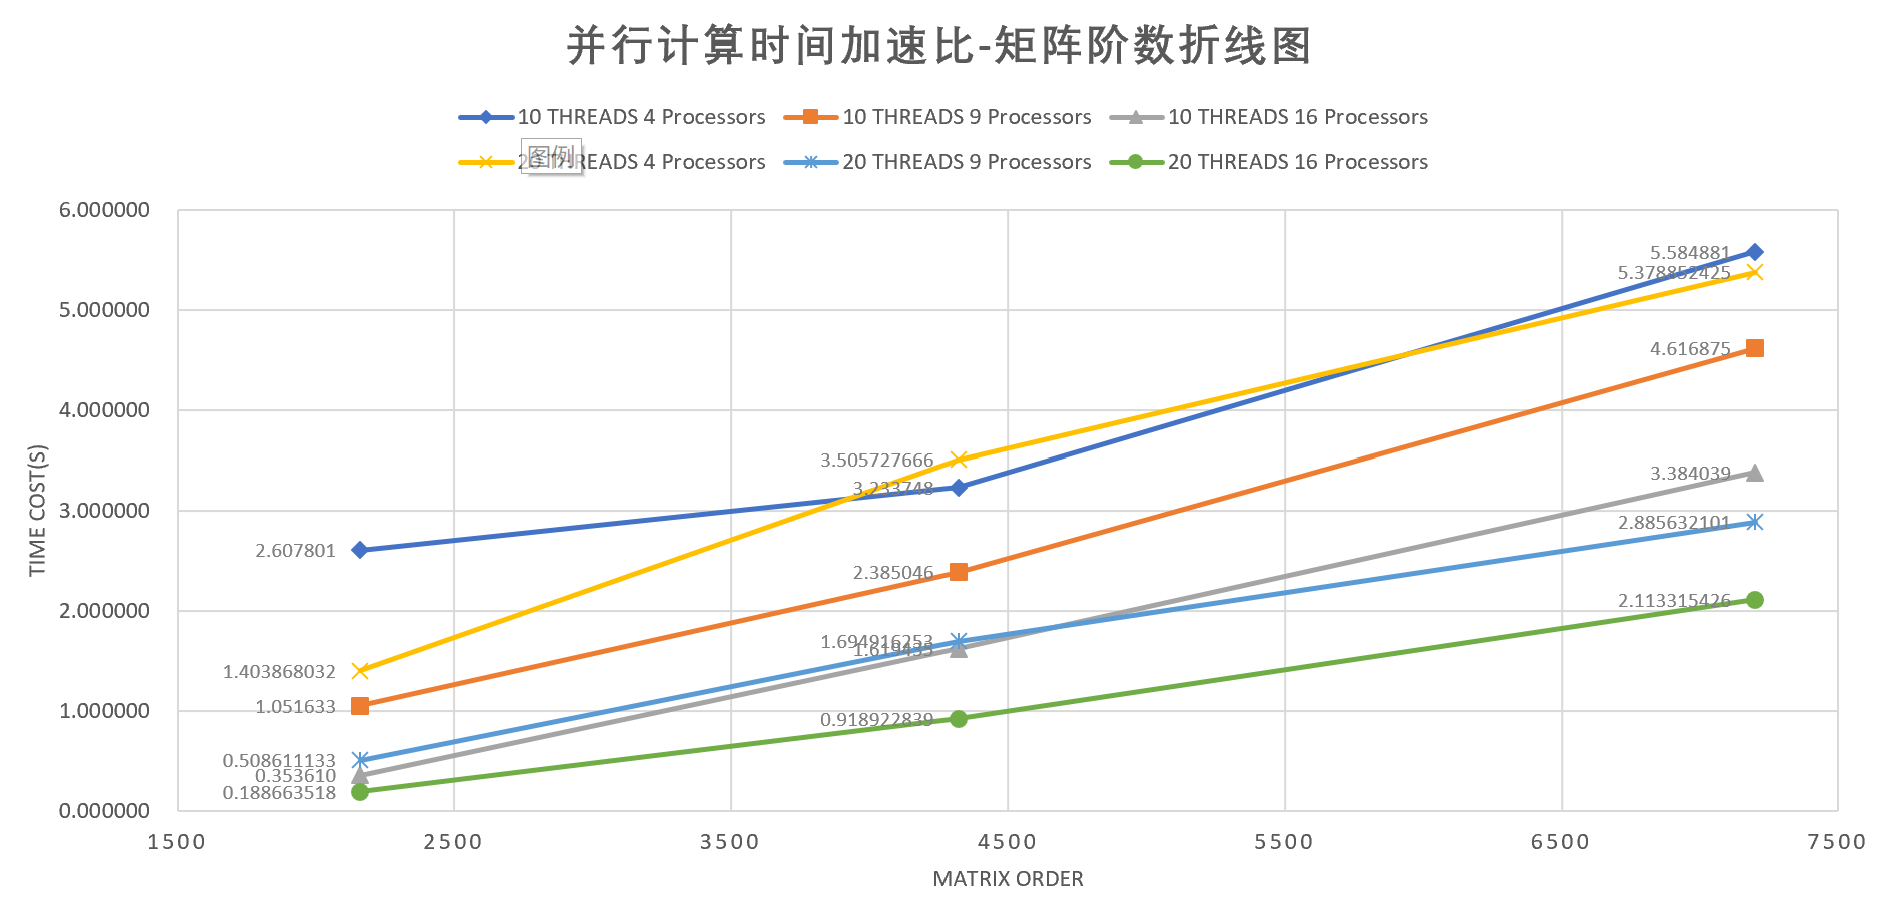
\includegraphics[width=0.8\textwidth]{pcr.png}
            \caption{并行通信时间折线图}
        \end{figure}

        \clearpage

\subsubsection{并行计算时间效率}

% Please add the following required packages to your document preamble:
% \usepackage{multirow}
% \usepackage[table,xcdraw]{xcolor}
% If you use beamer only pass "xcolor=table" option, i.e. \documentclass[xcolor=table]{beamer}
\begin{table}[h]
    \caption{并行计算时间效率表}
    \label{tab:my-table}
    \centering

    \begin{tabular}{|c|l|l|l|l|}
    \hline
    \multicolumn{5}{|c|}{efficiency}                                                                                                                                                           \\ \hline
    \multicolumn{1}{|l|}{}                                                  &            & \multicolumn{3}{c|}{MATRIX ORDER}                                                                   \\ \hline
    \multicolumn{1}{|l|}{}                                                  & Processors & 2160                            & 4320                            & 7200                            \\ \hline
                                                                            & 4          & {\color[HTML]{000000} 0.065195} & {\color[HTML]{000000} 0.080844} & {\color[HTML]{000000} 0.139622} \\ \cline{2-5} 
                                                                            & 9          & {\color[HTML]{000000} 0.011685} & {\color[HTML]{000000} 0.026501} & {\color[HTML]{000000} 0.051299} \\ \cline{2-5} 
    \multirow{-3}{*}{\begin{tabular}[c]{@{}c@{}}10 \\ THREADS\end{tabular}} & 16         & {\color[HTML]{000000} 0.00221}  & {\color[HTML]{000000} 0.010121} & {\color[HTML]{000000} 0.02115}  \\ \hline
                                                                            & 4          & {\color[HTML]{000000} 0.017548} & {\color[HTML]{000000} 0.043822} & {\color[HTML]{000000} 0.067236} \\ \cline{2-5} 
                                                                            & 9          & {\color[HTML]{000000} 0.002826} & {\color[HTML]{000000} 0.009416} & {\color[HTML]{000000} 0.016031} \\ \cline{2-5} 
    \multirow{-3}{*}{\begin{tabular}[c]{@{}c@{}}20 \\ THREADS\end{tabular}} & 16         & {\color[HTML]{000000} 0.00059}  & {\color[HTML]{000000} 0.002872} & {\color[HTML]{000000} 0.006604} \\ \hline
    \end{tabular}
    \end{table}
    \begin{figure}[h]
        \label{Ratio}
        \centering
            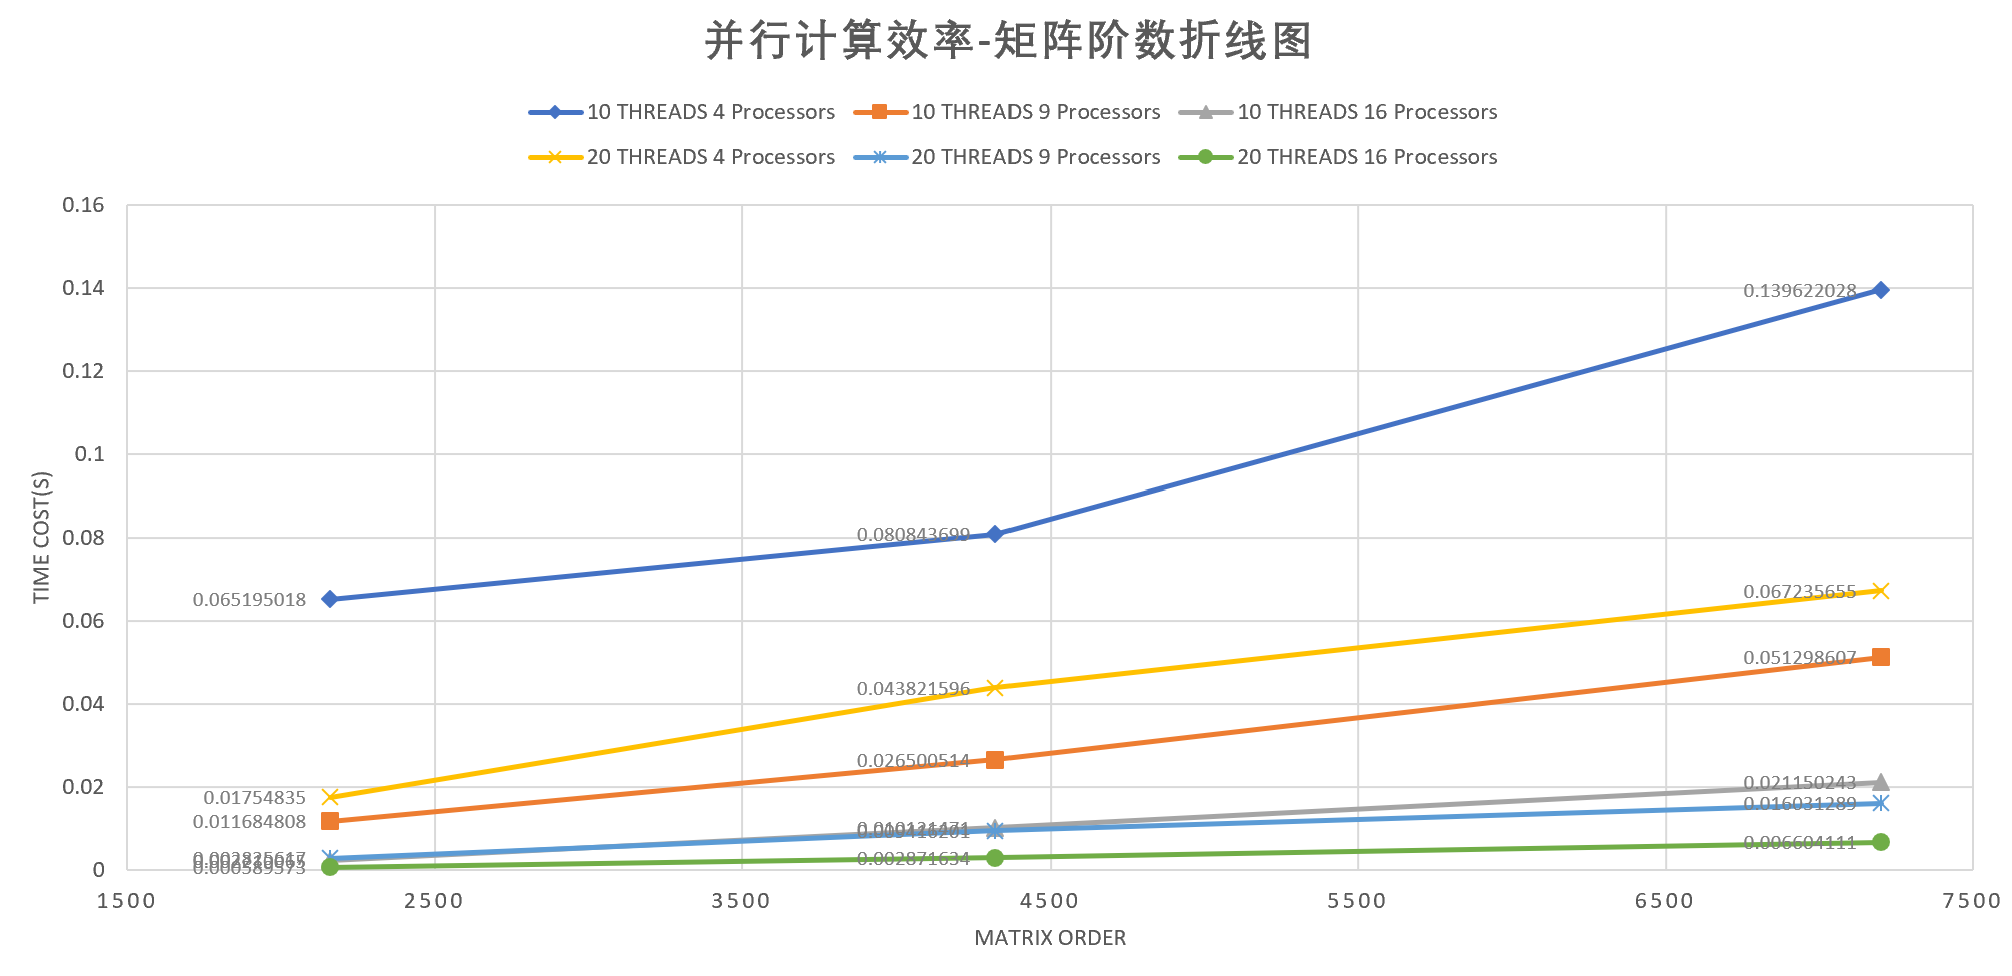
\includegraphics[width=0.8\textwidth]{eff.png}
            \caption{并行效率折线图}
        \end{figure}
        \clearpage

\subsection{两种算法对比}
在矩阵阶数为7200,处理器数为9的情况下,我对比了此前实现的算法与加入OMP后的算法。
其中Thread Count为1的数据即为此前算法,Thread Count不为1的是加入OMP后的算法。
\begin{table}[h]
    \caption{两种算法并行计算时间表}
    \label{tab:my-table}
    \centering

    \begin{tabular}{|l|l|}
    \hline
    Thread Count & PARALLEL CALC TIME \\ \hline
    1            & 0.020316           \\ \hline
    10           & 0.038875           \\ \hline
    20           & 0.062229           \\ \hline
    \end{tabular}
    \end{table}
    \begin{figure}[h]
        \label{Ratio}
        \centering
            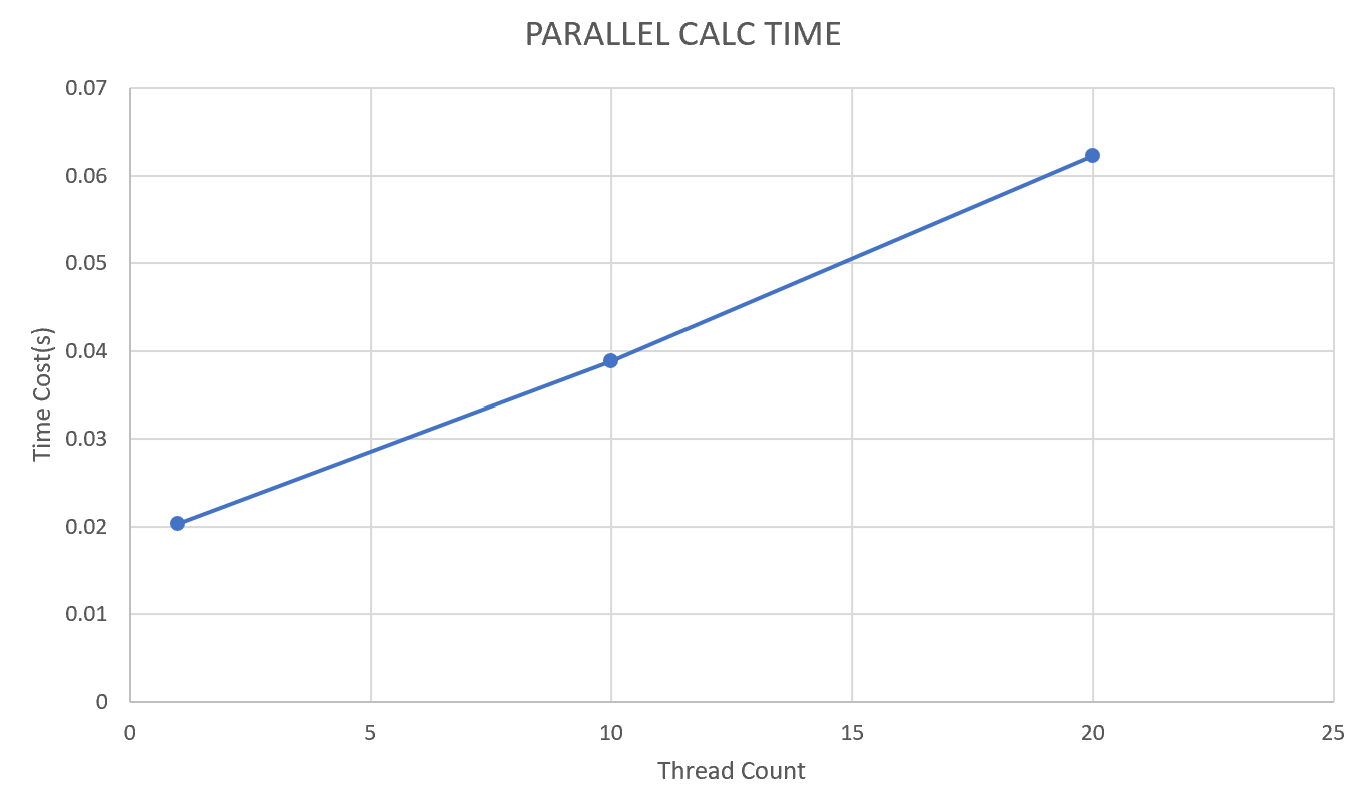
\includegraphics[width=0.8\textwidth]{cmpc.png}
            \caption{两种算法并行计算时间折线图}
        \end{figure}

        \begin{table}[h]
            \caption{两种算法并行总时间表}
            \centering

            \label{tab:my-table}
            \begin{tabular}{|l|l|}
            \hline
            Thread Count & PARALLEL ALL TIME \\ \hline
            1            & 0.835079          \\ \hline
            10           & 0.905315          \\ \hline
            20           & 0.9313            \\ \hline
            \end{tabular}
            \end{table}


                \begin{figure}[h]
                    \label{Ratio}
                    \centering
                        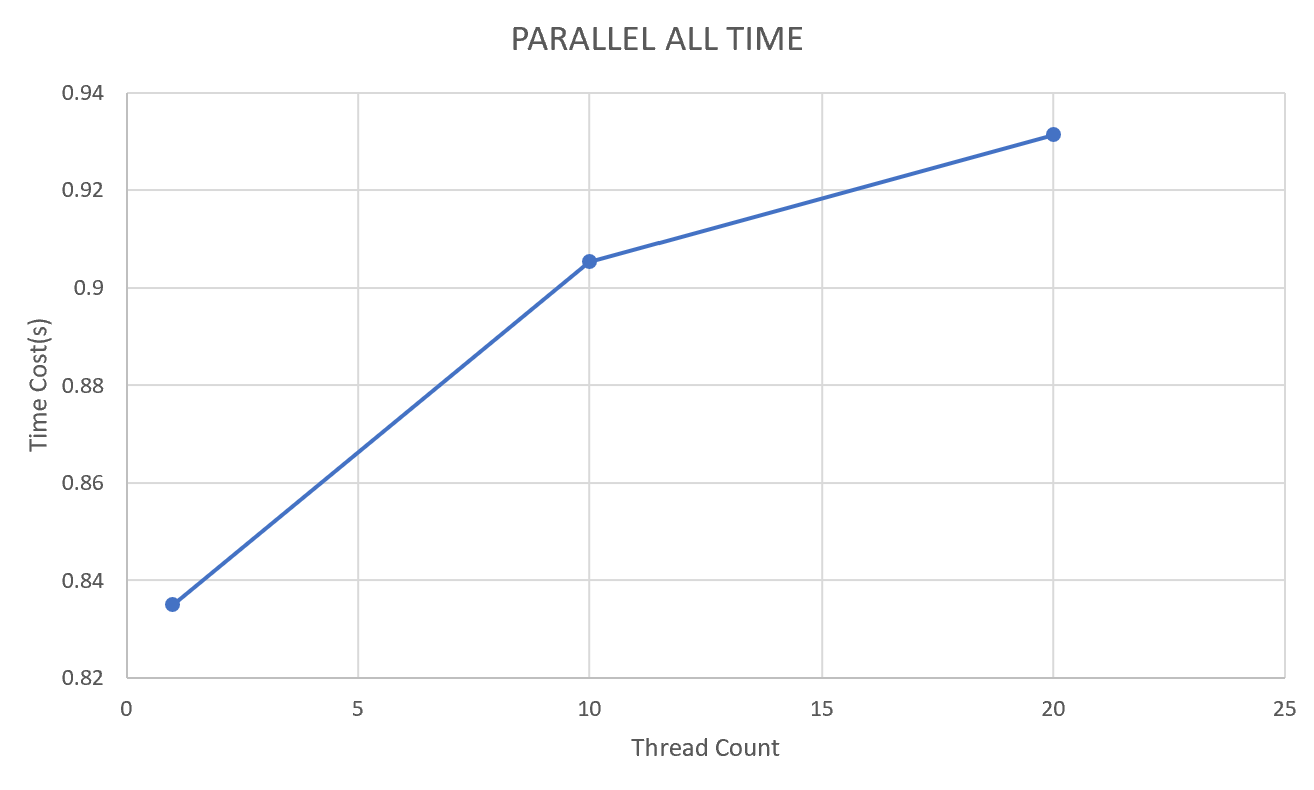
\includegraphics[width=0.8\textwidth]{cmpa.png}
                        \caption{两种算法并行总时间折线图}
                    \end{figure}
可能是由于测试的矩阵规模不够大,OMP在每个线程上并不能得到理想的加速结果,反而比
不采用OMP的版本用时更多(无论是计算时间还是总时间). 因此这也提醒了我,在实验规模
不大时,无须采用过多的并行技术。


\clearpage

\section{PA2}
本题在集群上的目录为/home/2018011423/HW5/PA2,在该文件夹下输入make即可编译,make run即可运行。

\subsection{}
私有的变量有i, j, count. 共享的变量有a, n, temp.
\subsection{}
没有循环依赖。每个线程之间彼此都使用私有的i, j, count,
对共享的temp数组的写操作也是彼此不重叠的,对a和n只存在读操作,
因此不存在依赖和冲突。
\subsection{}
可以并行化memcpy的调用。但是不一定能提高效率,
因为memcpy自身效率已经很高,开辟新线程还会带来额外的时间开销,因此不一定能够提高效率。

\subsection{}
程序的实现思路如下:我使用了题目中给出的计数排序的实现方式, 并利用parallel for语句对其加以
改造使其并行化。
\subsection{分析不同数据规模下,各排序算法的性能}
在这一部分,我将对比不同数据规模下,串行计数排序、并行计数排序、快速排序的性能。
此处的并行计数排序,我采用了10线程和默认调度方式。分析图表如下:
\begin{table}[h]
    \caption{各排序算法性能表}
    \label{tab:my-table}
    \centering
    \resizebox{16cm}{!} {
    \begin{tabular}{|l|l|l|l|l|l|l|l|}
    \hline
    array size                  & 100      & 500      & 1000     & 5000     & 10000    & 50000     & 100000    \\ \hline
    Serial Count Sort Time(s)   & 0.000120 & 0.003107 & 0.013448 & 0.202669 & 0.604671 & 13.615840 & 53.869850 \\ \hline
    Parallel Count Sort Time(s) & 0.000254 & 0.000705 & 0.002144 & 0.038180 & 0.116571 & 1.759016  & 6.806380  \\ \hline
    QuickSort Time(s)           & 0.000020 & 0.000216 & 0.000296 & 0.000545 & 0.001082 & 0.010681  & 0.022842  \\ \hline
    \end{tabular}}
    \end{table}
    \begin{figure}[h]
        \label{Ratio}
        \centering
            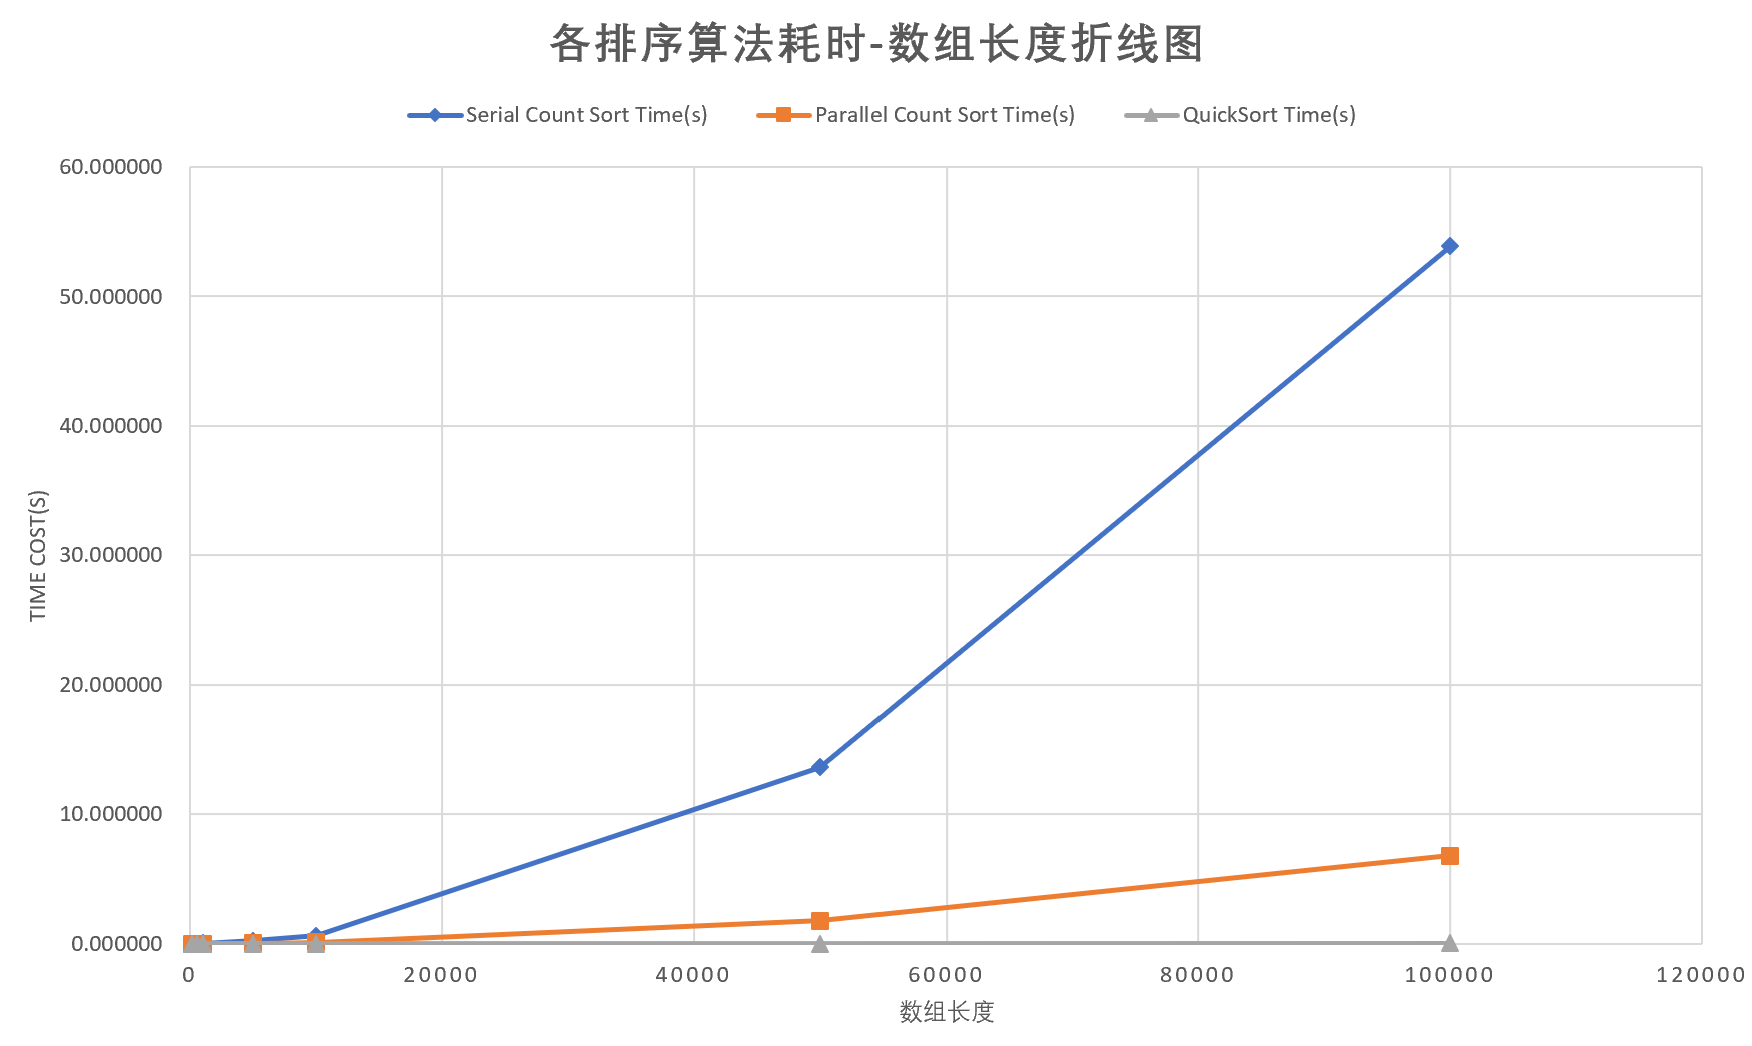
\includegraphics[width=0.8\textwidth]{sa.png}
            \caption{各排序算法耗时-数组长度折线图}
        \end{figure}
        \begin{table}[h]
            \caption{并行计数排序相较串行计数排序加速比}
            \label{tab:my-table}
            \centering
            \resizebox{16cm}{!}{
            \begin{tabular}{|l|l|l|l|l|l|l|l|}
            \hline
            array size   & 100         & 500         & 1000       & 5000        & 10000       & 50000       & 100000      \\ \hline
            SpeedUpRatio & 0.472440945 & 4.407092199 & 6.27238806 & 5.308250393 & 5.187147747 & 7.740600427 & 7.914610997 \\ \hline
            \end{tabular}}
            \end{table}

            \begin{figure}[h]
                \label{Ratio}
                \centering
                    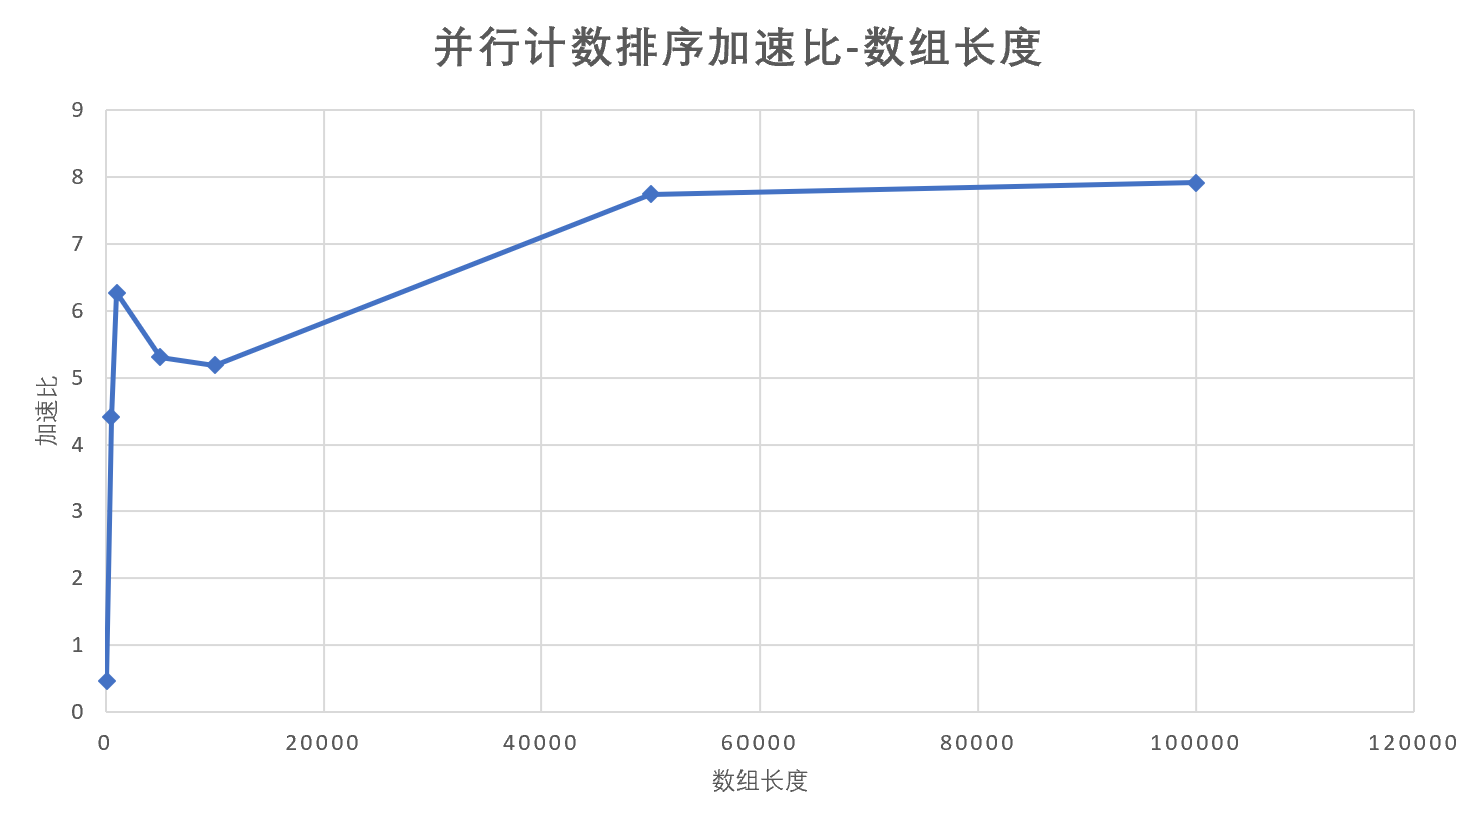
\includegraphics[width=0.8\textwidth]{psr.png}
                    \caption{并行计数排序加速比-数组长度折线图}
                \end{figure}
从图表中可以看出,相较串行计数排序,并行计数排序在数据规模较大时,表现出了较好的加速性能。
但是由于题中所给的计数排序时间复杂度为$O(n^2)$, 而快速排序时间复杂度为$O(nlogn)$, 其中n
为待排序的数组长度,因此两种计数排序的耗时都明显高于快速排序。

\clearpage
\subsection{不同调度策略下,程序运行效率}
\begin{table}[h]
    \caption{不同调度策略,程序耗时表}
    \label{tab:my-table}
    \resizebox{16cm}{!}{
    \begin{tabular}{|l|l|l|l|l|l|l|l|l|l|l|l|l|l|l|l|}
    \hline
                 & \multicolumn{5}{c|}{static}           & \multicolumn{5}{c|}{Dynamic}          & \multicolumn{5}{c|}{Guided}           \\ \hline
    Chunk Size   & 1     & 10    & 50    & 100   & 500   & 1     & 10    & 50    & 100   & 500   & 1     & 10    & 50    & 100   & 500   \\ \hline
    Time Cost(s) & 0.118 & 0.115 & 0.117 & 0.117 & 0.117 & 0.109 & 0.108 & 0.110 & 0.114 & 0.118 & 0.108 & 0.108 & 0.110 & 0.111 & 0.122 \\ \hline
    \end{tabular}}
    \end{table}


\begin{figure}[h]
    \label{Ratio}
    \centering
        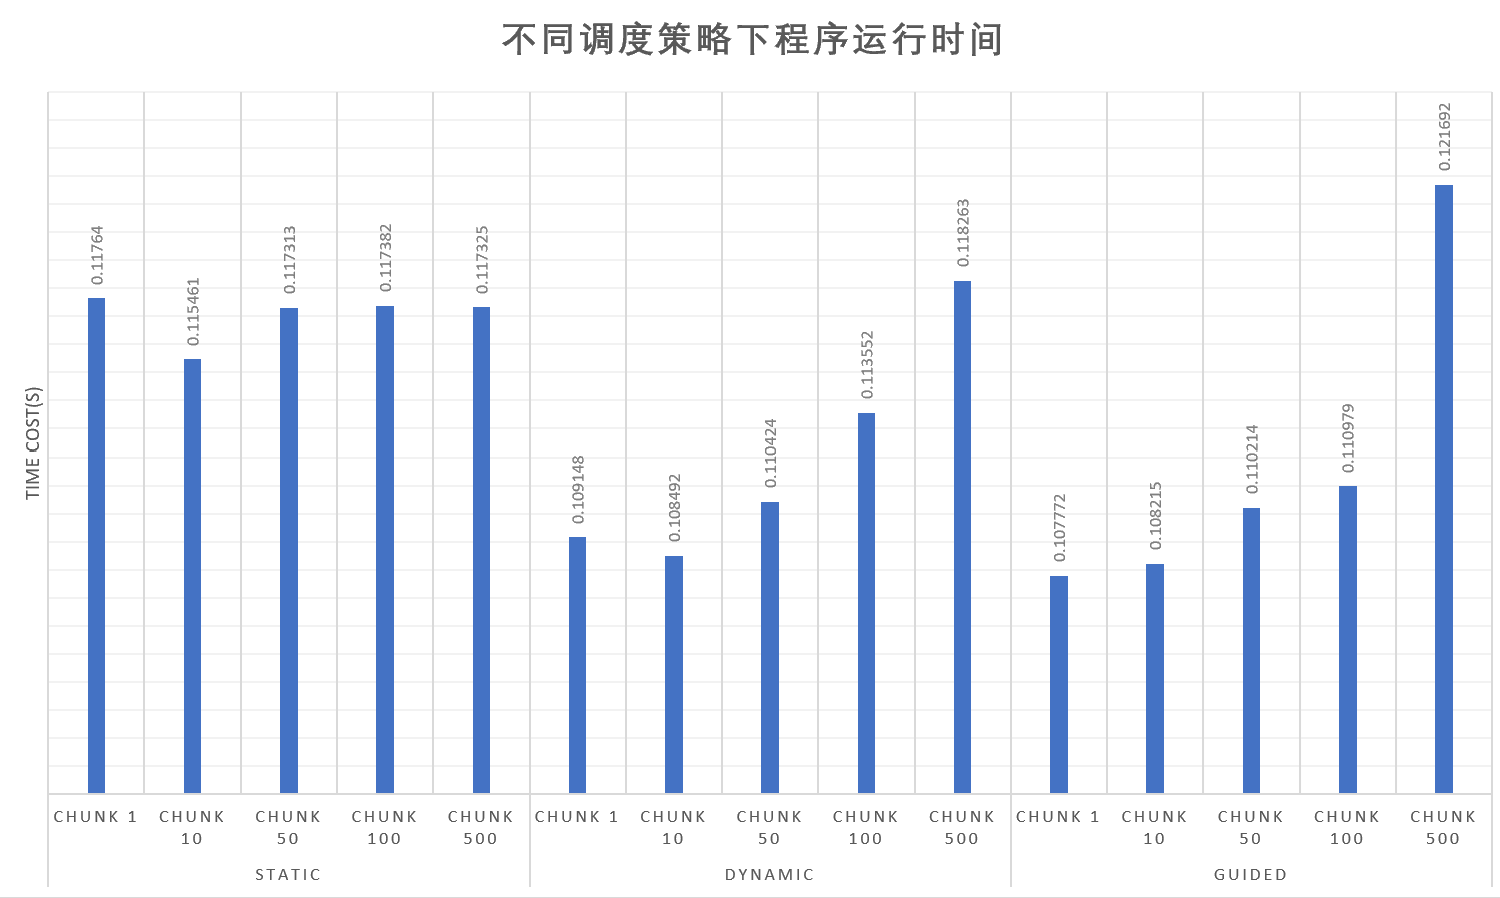
\includegraphics[width=0.8\textwidth]{st.png}
        \caption{不同调度策略下,程序运行时间柱状图}
    \end{figure}
理论上讲,在本题的场景中,分配到数组中的元素进行计数排序的时间成本应该不会有很大区别。
因此使用Static调度会是一个好的选择,Dynamic调度可能会因为动态调度而比Static调度慢一些。

但是从实际的实验结果来看,Dynamic调度耗时比Static调度略少,并且ChunkSize较小时运行速度更快。
在Static调度方法中,ChunkSize对耗时影响不大。而在Guided调度中,耗时随着ChunkSize的增大而增加。


\bibliographystyle{plain}
\bibliography{ref} %这里的这个ref就是对文件ref.bib的引用

\end{document}
